\clearpage
\section{Data}\label{sec:germ-electr-mark}

The focus of our study lies on quantifying the medium- to long-term investment potential for the German electricity market. Therefore, the following data was obtained: the initial available capacities in different technologies of each of the major players, the corresponding marginal and investment costs and the market demand for electricity.

\subsection{The German electricity market}

The German electricity market was liberalized in 1998 and is the largest in Europe with a gross production of 633.2 TWh in 2006 \citep{IEA2007}. More than half of the power is generated with coal, other major sources are nuclear and gas. The German power market is dominated by a few large players (E.ON, RWE, EnBW, Vattenfall). These firms are transmission system operators and own 90\% of total generation capacity. \cite{Brunekreeft2006} report values for the Herfindahl Hirschman Index (HHI)\footnote{This is a common measure of market power and is calculated as sum of the squared market shares in an industry.} of over 2000. Electricity distribution is organized by approximately 900 communal distributors. The German energy market regulator  \emph{Bundesnetzagentur} was installed in 2005. There are several interesting developments on the German electricity market. For example, new capacities are urgently needed as Germany decided on a phase-out of nuclear power generation by 2020 \citep[see e.g.][]{IEA2007a}. In addition to that, a large stake of the existing generation capacities are close to the end of its service life. The \emph{German Energy Agency} estimates that investments in generation capacity of up to 40,000 MW will be necessary in the upcoming years. This, together with a tendency towards more environmental-friendly technologies supports the importance of exploring investment incentives in an oligopolistic market under uncertainity.
 
In recent years, the price levels on German wholesale electricity markets have risen as reported by \cite{Weigt2007}, who attribute this development to market power. In a similar vein, \cite{Brunekreeft2005} argue that this price increase is now exercised on wholesale markets as transmission tariffs, which increases the regulatory pressure on the vertically integrated major players on the market.

\subsection{Available capacities}
\label{sec:available-capacities}

Apart from that, our analysis will abstract from vertical relationships and transmission constraints. According to \cite{IEA2007a}, there are no significant congestions within Germany. Cross boarder transfer capacities and congestions are given in table \ref{tab:transfer} and help us to determine the relevant market. There seems to be no congestion at all between Germany and Austria, so we include the Austrian demand and fringe supply into our analysis. The heavily congested lines to Denmark and The Netherlands suggest that exports from Germany to the latter countries take place at maximum capacities almost all over the year, so we subtract the respective exports from the German supply. French and Czech capacities are added to the non-strategic fringe but only up to their import capacity constraints.

\begin{table}[htb]
\centering
\small
\caption{Available transfer capacities (Winter 2006/07) and cross-border congestion (Jan-May 2005)}
\vspace{0.3cm}
\begin{tabular}{lrrrrr}
\hline
           &            & \multicolumn{ 2}{c}{to Germany} & \multicolumn{ 2}{c}{from Germany} \\
\hline
           &            & Capacities  & Share of hours  & Capacities & Share of hours  \\

           &            & in MW        &  congested & in MW           &  congested \\
\hline
\hline
   Austria &            &       1,400 &        0\% &       1,600 &        0\% \\

Czech Republic &            &       2,260 &       68\% &        700 &       36\% \\

    France &            &       2,850 &       33\% &       3,300 &       41\% \\

The Netherlands &            &       3,000 &       64\% &       3,800 &       90\% \\

   Denmark &            &       1,750 &            &       1,350 &      100\% \\

\hline
\end{tabular}  
\label{tab:transfer}
\\
\vspace{0.3cm}
\scriptsize Source: \cite{IEA2007a}
\end{table}

Figure \ref{fig:capacities} gives an overview about the existing installed capacity and the different production technologies on the German electricity market.

% \begin{table}[htb]
% \centering
% \small
% \caption{Installed capacities in MW of major players in Germany}
% \vspace{0.3cm}
% \begin{tabular}[htb]{crrrrrrrrr}
% \hline
%            &      Hydro &    Nuclear &  Lignite &  Hardcoal &        Gas &        Oil &     Pump \\
% \hline\hline
%        RWE &        741 &       5,499 &      10,554 &       7,249 &       4,297 &        188 &        793 \\

%       E.ON &       1,320 &       8,473 &       1,425 &       9,461 &       3,808 &       1,779 &       1,110 \\

% Vattenfall &          9 &       1,421 &       6,932 &       1,729 &        870 &       1,429 &       2,883 \\

%       EnBW &        447 &       4,272 &        453 &       3,288 &       1,083 &        617 &        368 \\
      
%        Fringe &	12444 &	557  &	428  & 	 8496	 & 12615  &	1715  &	2109 \\

% \hline
% \end{tabular} 
% \label{tab:capacities}
% \\
% \vspace{0.3cm}
% \scriptsize Source: \cite{Ellersdorfer2005}
% \end{table}

\begin{figure}[htb]
  \centering
\caption{Installed capacities in GW of major players in Germany}
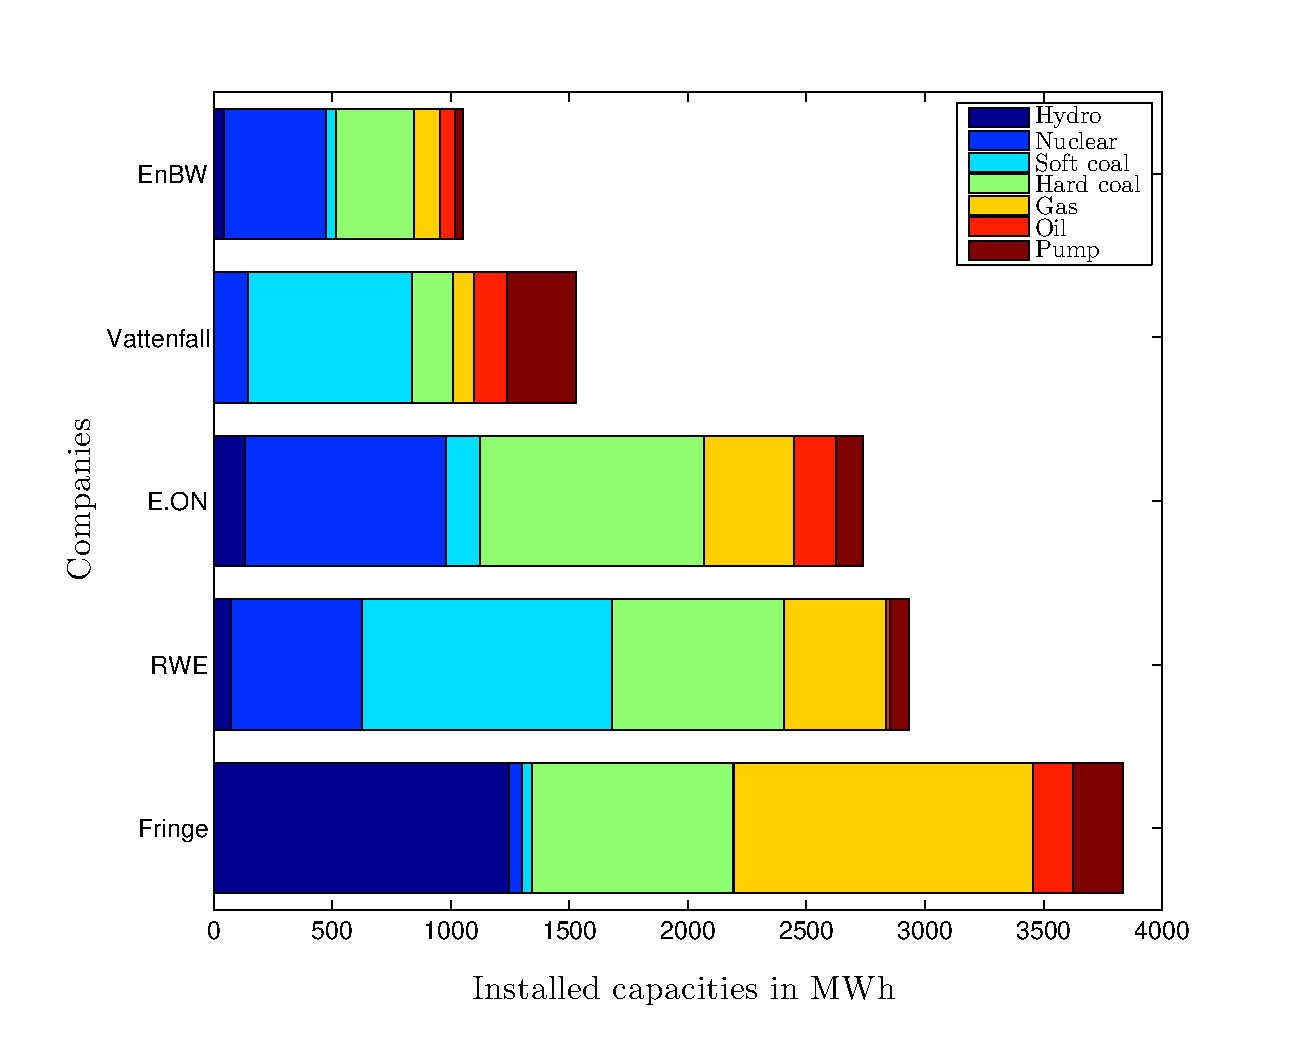
\includegraphics[width=0.8\textwidth]{numericalpaper/capacities}
  \label{fig:capacities}
\\
 \scriptsize Source: \cite{Ellersdorfer2005}
\end{figure}

\clearpage
\subsection{Market demand and electricity prices}
\label{sec:mark-demand-electr}

Information about the hourly electricity load can be obtained from \cite{UCTE2006}. The data in figure \ref{fig:load} shows the typical daily and seasonal patterns of electricity demand.

\begin{figure}[htb]
  \centering
\caption{Hourly load values in Austria and Germany for 2006 (in GWh)}
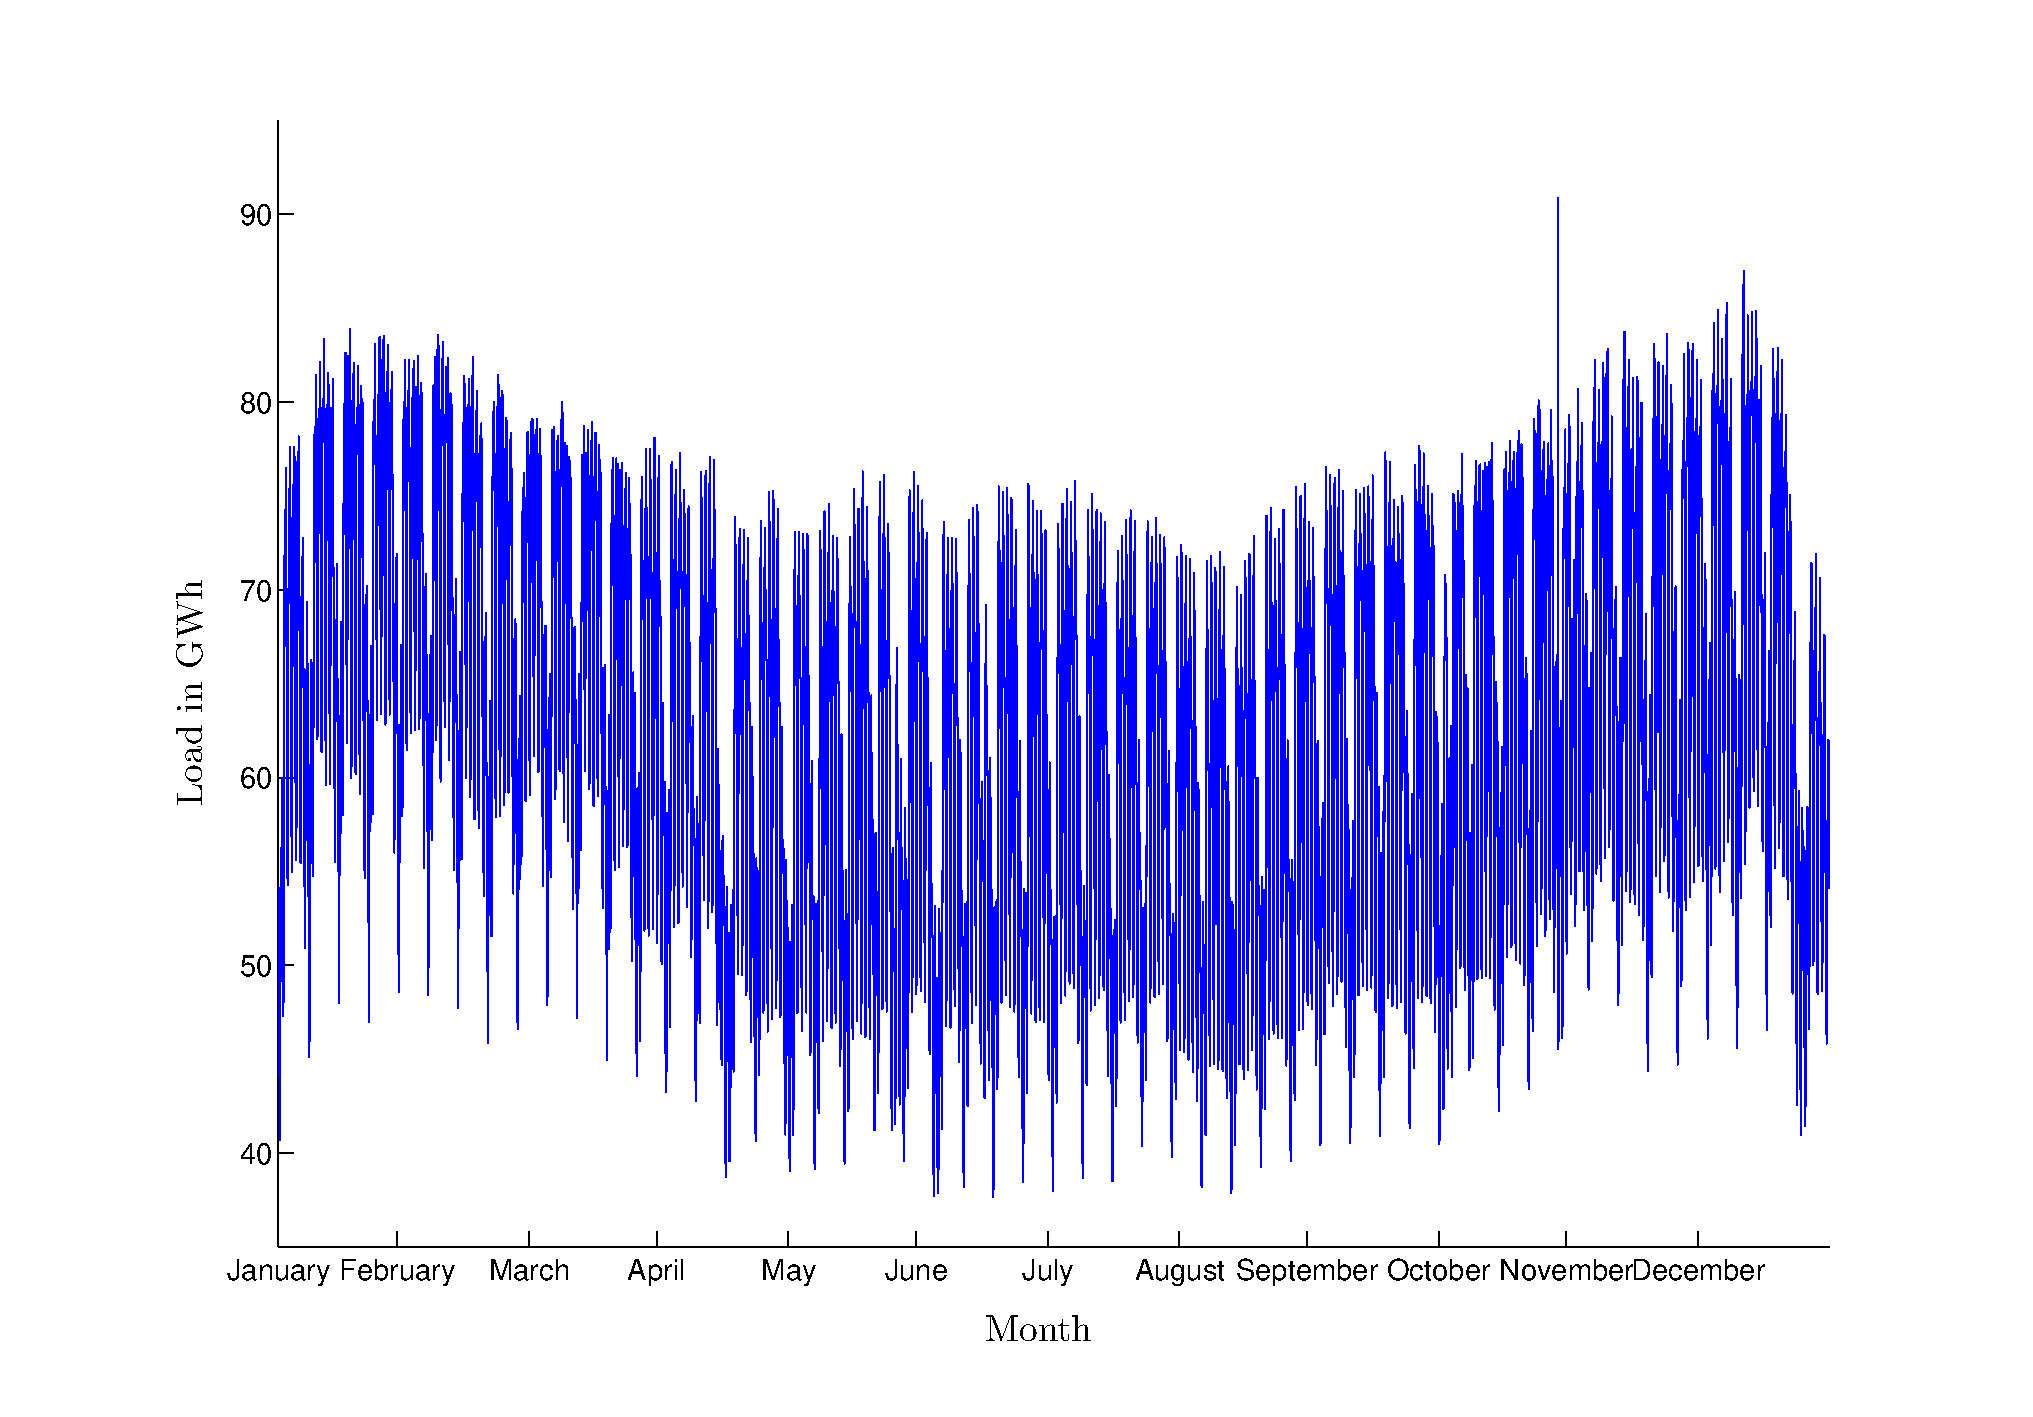
\includegraphics[width=0.8\textwidth]{numericalpaper/loadvalues}
  \label{fig:load}
\\
 \scriptsize Source: \cite{UCTE2006}
\end{figure}


The major stake of electricity trading is done on over-the-counter (OTC) markets for which it is hard to obtain data. However, the European Energy Exchange (EEX) gains more and more importance. Market participants can bid in day-ahead hourly contract auctions, or can trade block contracts and emission permits in continuous trading. Prices from the EEX can be used as a good approximation for the wholesale price of electricity. Plotting the prices against the trading volumes does not show a strong correlation. We see the expected positive relationship when comparing the exchange prices to the actual electricity demand per hour, see figure \ref{fig:pricequant}.

\begin{figure}[htb]
  \centering
\caption{Price-quantity relationship}
  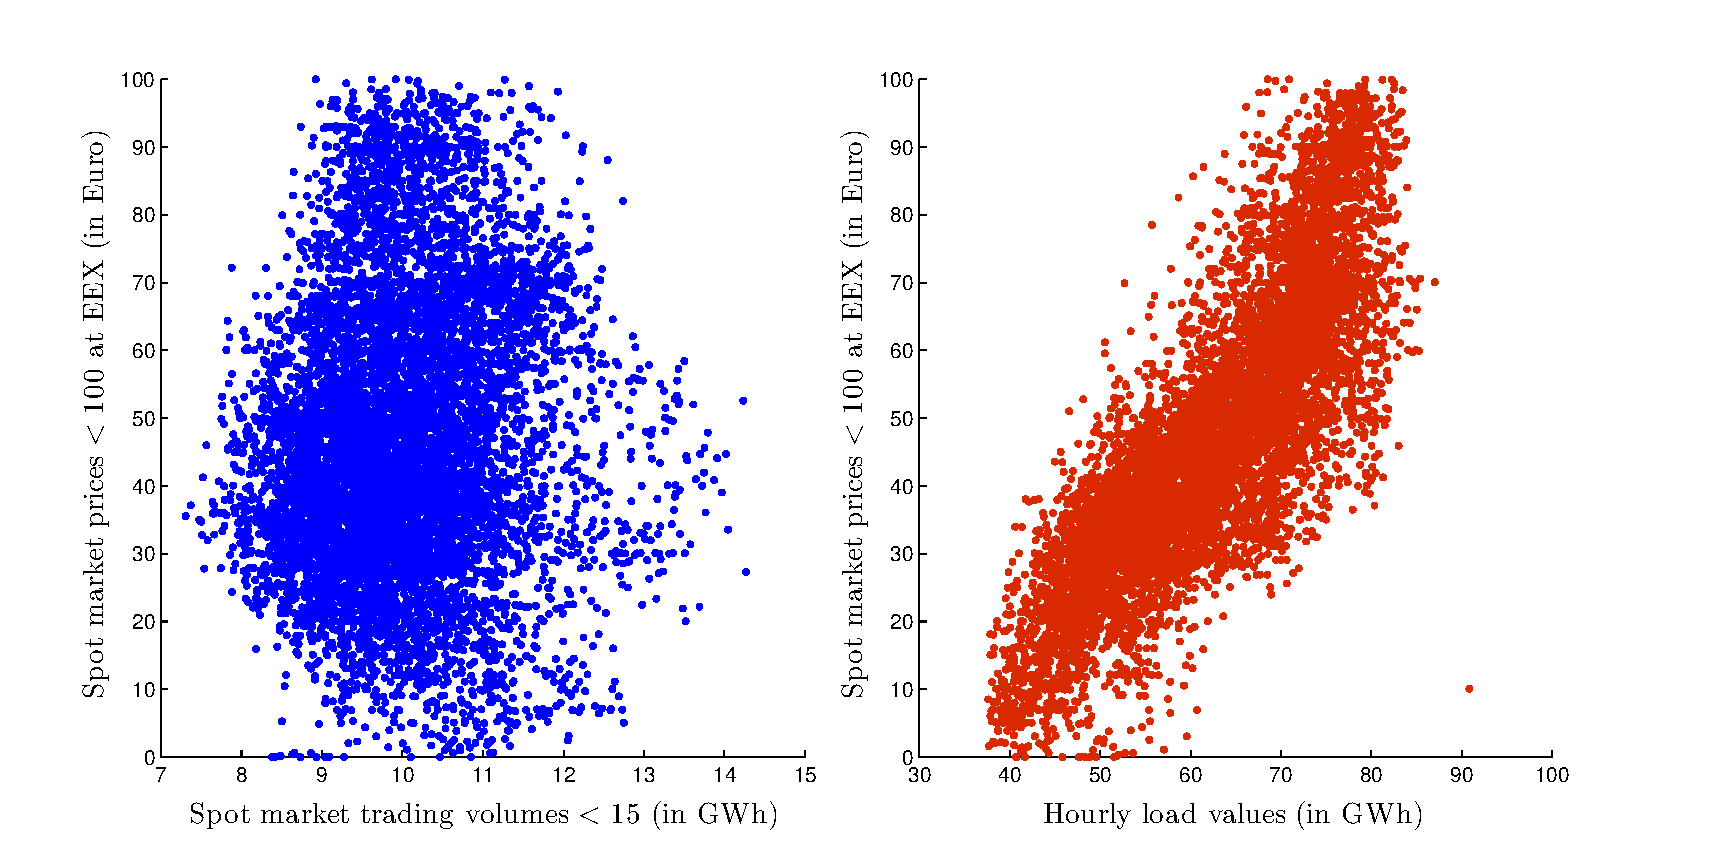
\includegraphics[width=0.9\textwidth]{numericalpaper/pricequant}
  \label{fig:pricequant}
\\
 \scriptsize Source: \cite{EEX2006, UCTE2006}
\end{figure}

To account for different states of the market, we separated the price-quantity combinations which occurred within a year by prices. As can be seen in table \ref{tab:marketsegments}, markets with extremely high prices occur only seldomly and prices between 20 and 40 are most common.

For each of the six states in which the market might be, we created linear demand functions based on average prices and quantities in these states. Note, that we also model the high-price market segment, to include price spikes which are a stylized fact of electricity prices.  To construct demand curves, \cite{Neuhoff2005} use a demand elasticity of 0.1, whereby \cite{Genc2007} argue that 0.2 is more commonly used to simulate the electricity market. As we have a more long run focus, we decided to use the latter value. It might be argued, that electricity demand is completely inelastic, as maybe only a very few industrial clients reduce their demand when prices rise. In response to that, \cite{Bushnell2003} notes that imports and exports provide some elasticity.

\begin{table}[ht]
\centering
\caption{Market segments}\label{tab:marketsegments}
\begin{tabular}{rrrrr}
  \hline
Price & Average price  & Average quantity & Number of & Percentage of \\
intervals& (Euro/MWh) &  (MWh) &  prices & of total prices\\
  \hline\hline
$0\leq p<20$ & 12.67 & 46,111.63 & 611 & 6.98\% \\
$20\leq p<40$ & 31.35 & 54,103.50 & 3,003 & 34.28\% \\
$40\leq p<60$ & 49.00 & 64,806.04 & 2,626 & 29.98\% \\
$60\leq p<80$ & 68.46 & 72,385.56 & 1,588 & 18.13\% \\
$80\leq p<100$ & 88.40 & 75,991.21 & 665 & 7.59\% \\
$100\leq p<\infty$& 176.06 & 76,482.34 & 266 & 3.04\% \\
   \hline
\end{tabular}
\\
\vspace{0.3cm}
\scriptsize Source: \cite{EEX2006, UCTE2006}
\end{table}

\clearpage
\subsection{Marginal and investment costs}
\label{sec:marg-investm-costs}

Data concerning the short run marginal costs and investment costs per MWh were obtained from \cite{Auer2006} and are shown in table \ref{tab:costs}. For pump storage plants we used the real option value of peak load electricity, which we approximated by the average option price for peak load electricity at the EEX in the year 2006. We do not provide fixed costs for pump hydropower and oil plants. In the case of hydropower plants construction costs depend heavily on the respective sites and therefore such costs are hard to estimate. Furthermore, all available sites for significant hydropower capacities in Central Europe seem to be occupied already. Oil fired plants are not considered a relevant investment option, because oil prices are just too high. The fixed investment costs can also be interpreted as present value of future yearly costs of capital.

\begin{table}[htb]
\centering
\caption{Variable and investment costs}
\vspace{0.3cm}
\begin{tabular}{rrr}
\hline
           & Variable costs & Investment costs\\
           &  (Euro/MWh)    &  (Euro/GW) \\
\hline\hline
     Hydro &        7.6 &    3,500\\

   Nuclear &        9.5 &    1,841 \\

   Lignite &       10.6 &    1,074 \\

 Hard coal &       16.1 &     971 \\

 Gas (CCGT) &       33.5 &     460 \\

Oil & 44            &   n/a\\

Pump &         80 &       n/a\\
\hline
\end{tabular}
\label{tab:costs}
\\
\vspace{0.3cm}
\scriptsize Source: \cite{Auer2006}
\end{table}



%%% Local Variables: 
%%% mode: latex
%%% TeX-master: "gencapinvest"
%%% End: 
